\chapter*{Summary}
Near field communication (NFC) allows two electronic devices to communicate wirelessly by bringing them close to each other. NFC has become widely used in applications such as personal electronics, industrial, medical, fitness and much more. There were already more than 500 million NFC-enabled devices in 2015 \cite{Texas2015}, and this number has only increased since then. 

The RF430CL330H Dynamic NFC Interface Transponder chip uses this technology to communicate over radio frequency, as well to having an $I^2C$ interface. Allowing the possibility for adding a diagnostic interface to configure and retrieve data from a host system. This report explains the procedure to design a PCB containing the RF430CL330H and evaluates the chip using an EVM (evaluation module) offered by Texas Instruments. The design is then integrated into a larger system. 
\begin{figure}[h]
\begin{center}
\center
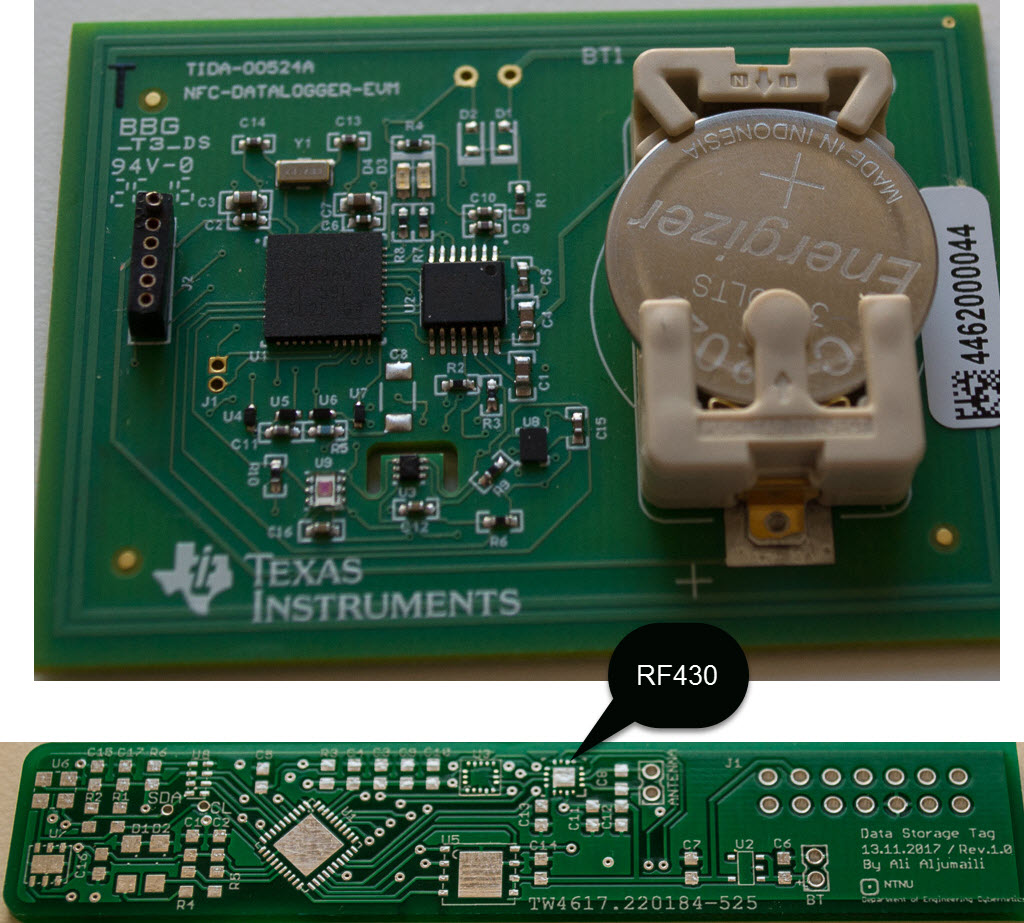
\includegraphics[scale=0.8]{Illustrations/summary.jpg}  
\caption{Evaluation kit and prototype}
\label{prototype}
\end{center}
\end{figure}
